%************************************************
\chapter[Appendix 6.1: Chapter 6 - Physiological response curves]{Appendix 6.1: Chapter 6 - Physiological response curves and additional results}\label{ch:environment_appendix}
%************************************************
\renewcommand{\thefigure}{A.6.1.\arabic{figure}}
\setcounter{figure}{0}

\renewcommand{\thetable}{A.6.1.\arabic{table}}
\setcounter{table}{0}

We modelled the physiological response of species to a non-resource environmental factor following the conceptual hypothesis of \cite{Maestre2009}, who assumed that plant species are ordered on a continuum ranging from pure competitors to pure stress-tolerants. Species were able to randomly colonize locations alongside an environmental gradient with varying levels of both non-resource and resource environmental factors (Fig. \ref{fig:figApp6.1.1}). Competitive species survive and grow best in optimal conditions, but are very sensitive to environmental stress. Stress-tolerant species, on the other hand, maintain moderate levels of survival and growth for higher stress levels.

For implementing this framework, we derived a flexible function able to reproduce different functional responses. The function is

\begin{equation} \label{eq:eqApp6.1.1}
P(x) = \frac{k * p_0 * e^{r_1 x}}{k + p_0 * e^{r_1 x -1}} - c(e^{r_2 x -1})
\end{equation}

where P(x) is the response variable, that in our scenario corresponds to survival or growth probability. The parameterisation we obtained for the species at the ends of the continuum, mimicking Fig. 1 of \cite{Maestre2009}, is given in Table \ref{tab:tabApp6.1.1}. With that parameterisation at the extreme behaviours, we generated 20 response curves for model species (Fig. \ref{fig:figApp6.1.2}), such that the transition between pure competitors and pure stress tolerant species is smooth, and all species have maximum survival probability in the absence of environmental stress.

\begin{table}[]
\caption[Response curves parameterization]{\color{Gray}Parameterisation of \ref{eq:eqApp6.1.1} for purely competitive and purely stress-tolerant species. Intermediate species have parameters within these ranges in all cases.}\label{tab:tabApp6.1.1}
\begin{tabular}{lllll}
\hline
  & \multicolumn{2}{l}{survival} & \multicolumn{2}{l}{growth}   \\
\hline
      & stress-tolerant & competitor    & stress-tolerant & competitor \\
k     & 1               & 0.1           & 0.7             & 0.1          \\
$p_0$ & 1               & 1             & 0.7             & 1          \\
$r_1$ & 0.1             & 0.01          & 0.1             & 0.05          \\
$r_2$ & 1               & 0.85          & 0.5             & 0.5          \\
c     & $3*10^{-5}$     & $3*10^{-4}$   & $5*10^{-3}$     & 0.05
\end{tabular}

\end{table}

\begin{figure}[!ht]
\centering
\includegraphics[width=.5\textwidth]{./Figures/Appendix6_1/Fig_1.png}
\caption[Environmental grid]{\color{Gray} A series of locations with linearly varying conditions of a resource factor (represented by circle size) and non-resource factor (from light to dark blue). The grid represented in this figure is of size 20*20, whereas the one used in the model is of size 50*50.}
\label{fig:figApp6.1.1}
\end{figure}

\begin{figure}[!ht]
\centering
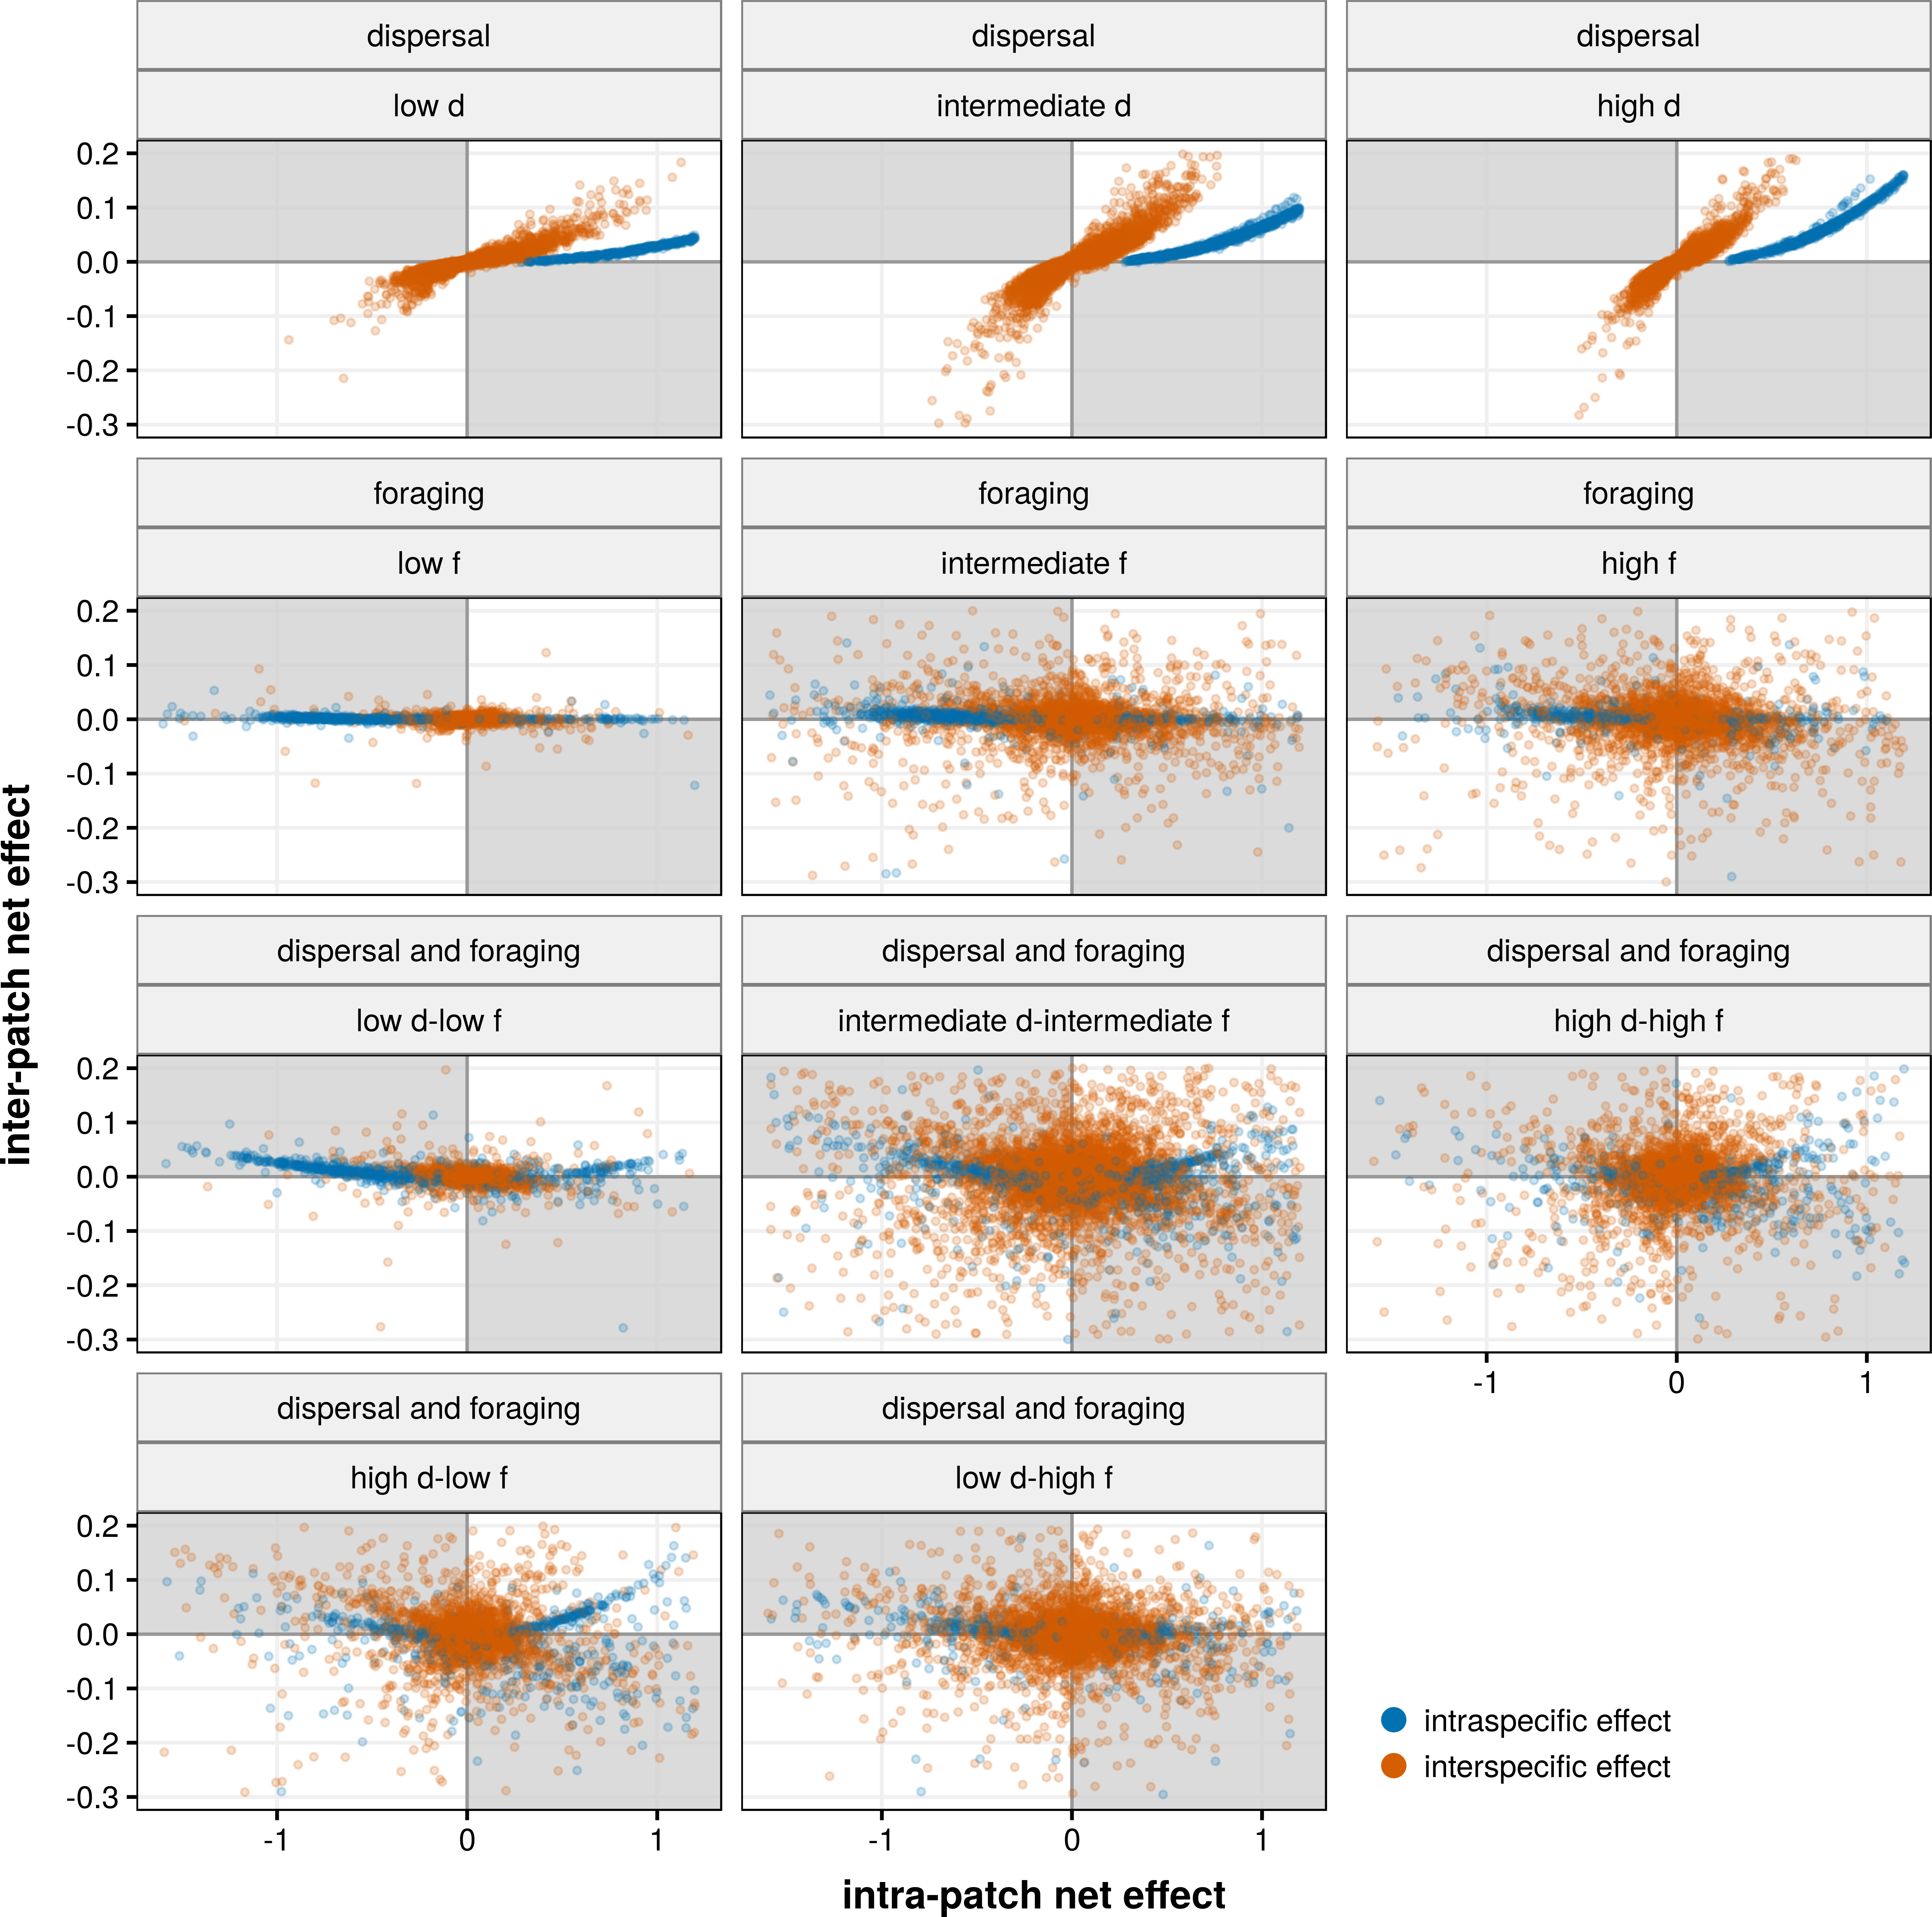
\includegraphics[width=\textwidth]{./Figures/Appendix6_1/Fig_2.png}
\caption[Response curves]{\color{Gray} Physiological response curves of 20 modelled species to a single non-resource environmental factor. Probabilities of survival (left panel) and growth (right panel) are modelled, and species range from purely stress-tolerant (dark blue curves) to purely competitive (yellow curves). Stress-tolerant species maintain a high probability of survival under a higher range of environmental stress, and also keep a moderate growth probability for longer than competitive species. The latter, on the other hand, are very sensitive to environmental stress, but grow better than stress-tolerant species under ideal conditions. These functional responses are adapted from Fig. 1 of \cite{Maestre2009}}
\label{fig:figApp6.1.2}
\end{figure}

\begin{figure}[!ht]
\centering
\includegraphics[width=\textwidth]{./Figures/Appendix6_1/Fig_3.png}
\caption[Two-dimensional community variability]{\color{Gray} Variation in community-level properties across the two dimensional gradient. As we are not interested in absolute values but rather in trends of variation, values in all panels are normalised, ranging from 0 (minimum values, dark blue) to 1 (maximum values, yellow).}
\label{fig:figApp6.1.3}
\end{figure}

\begin{figure}[!ht]
\centering
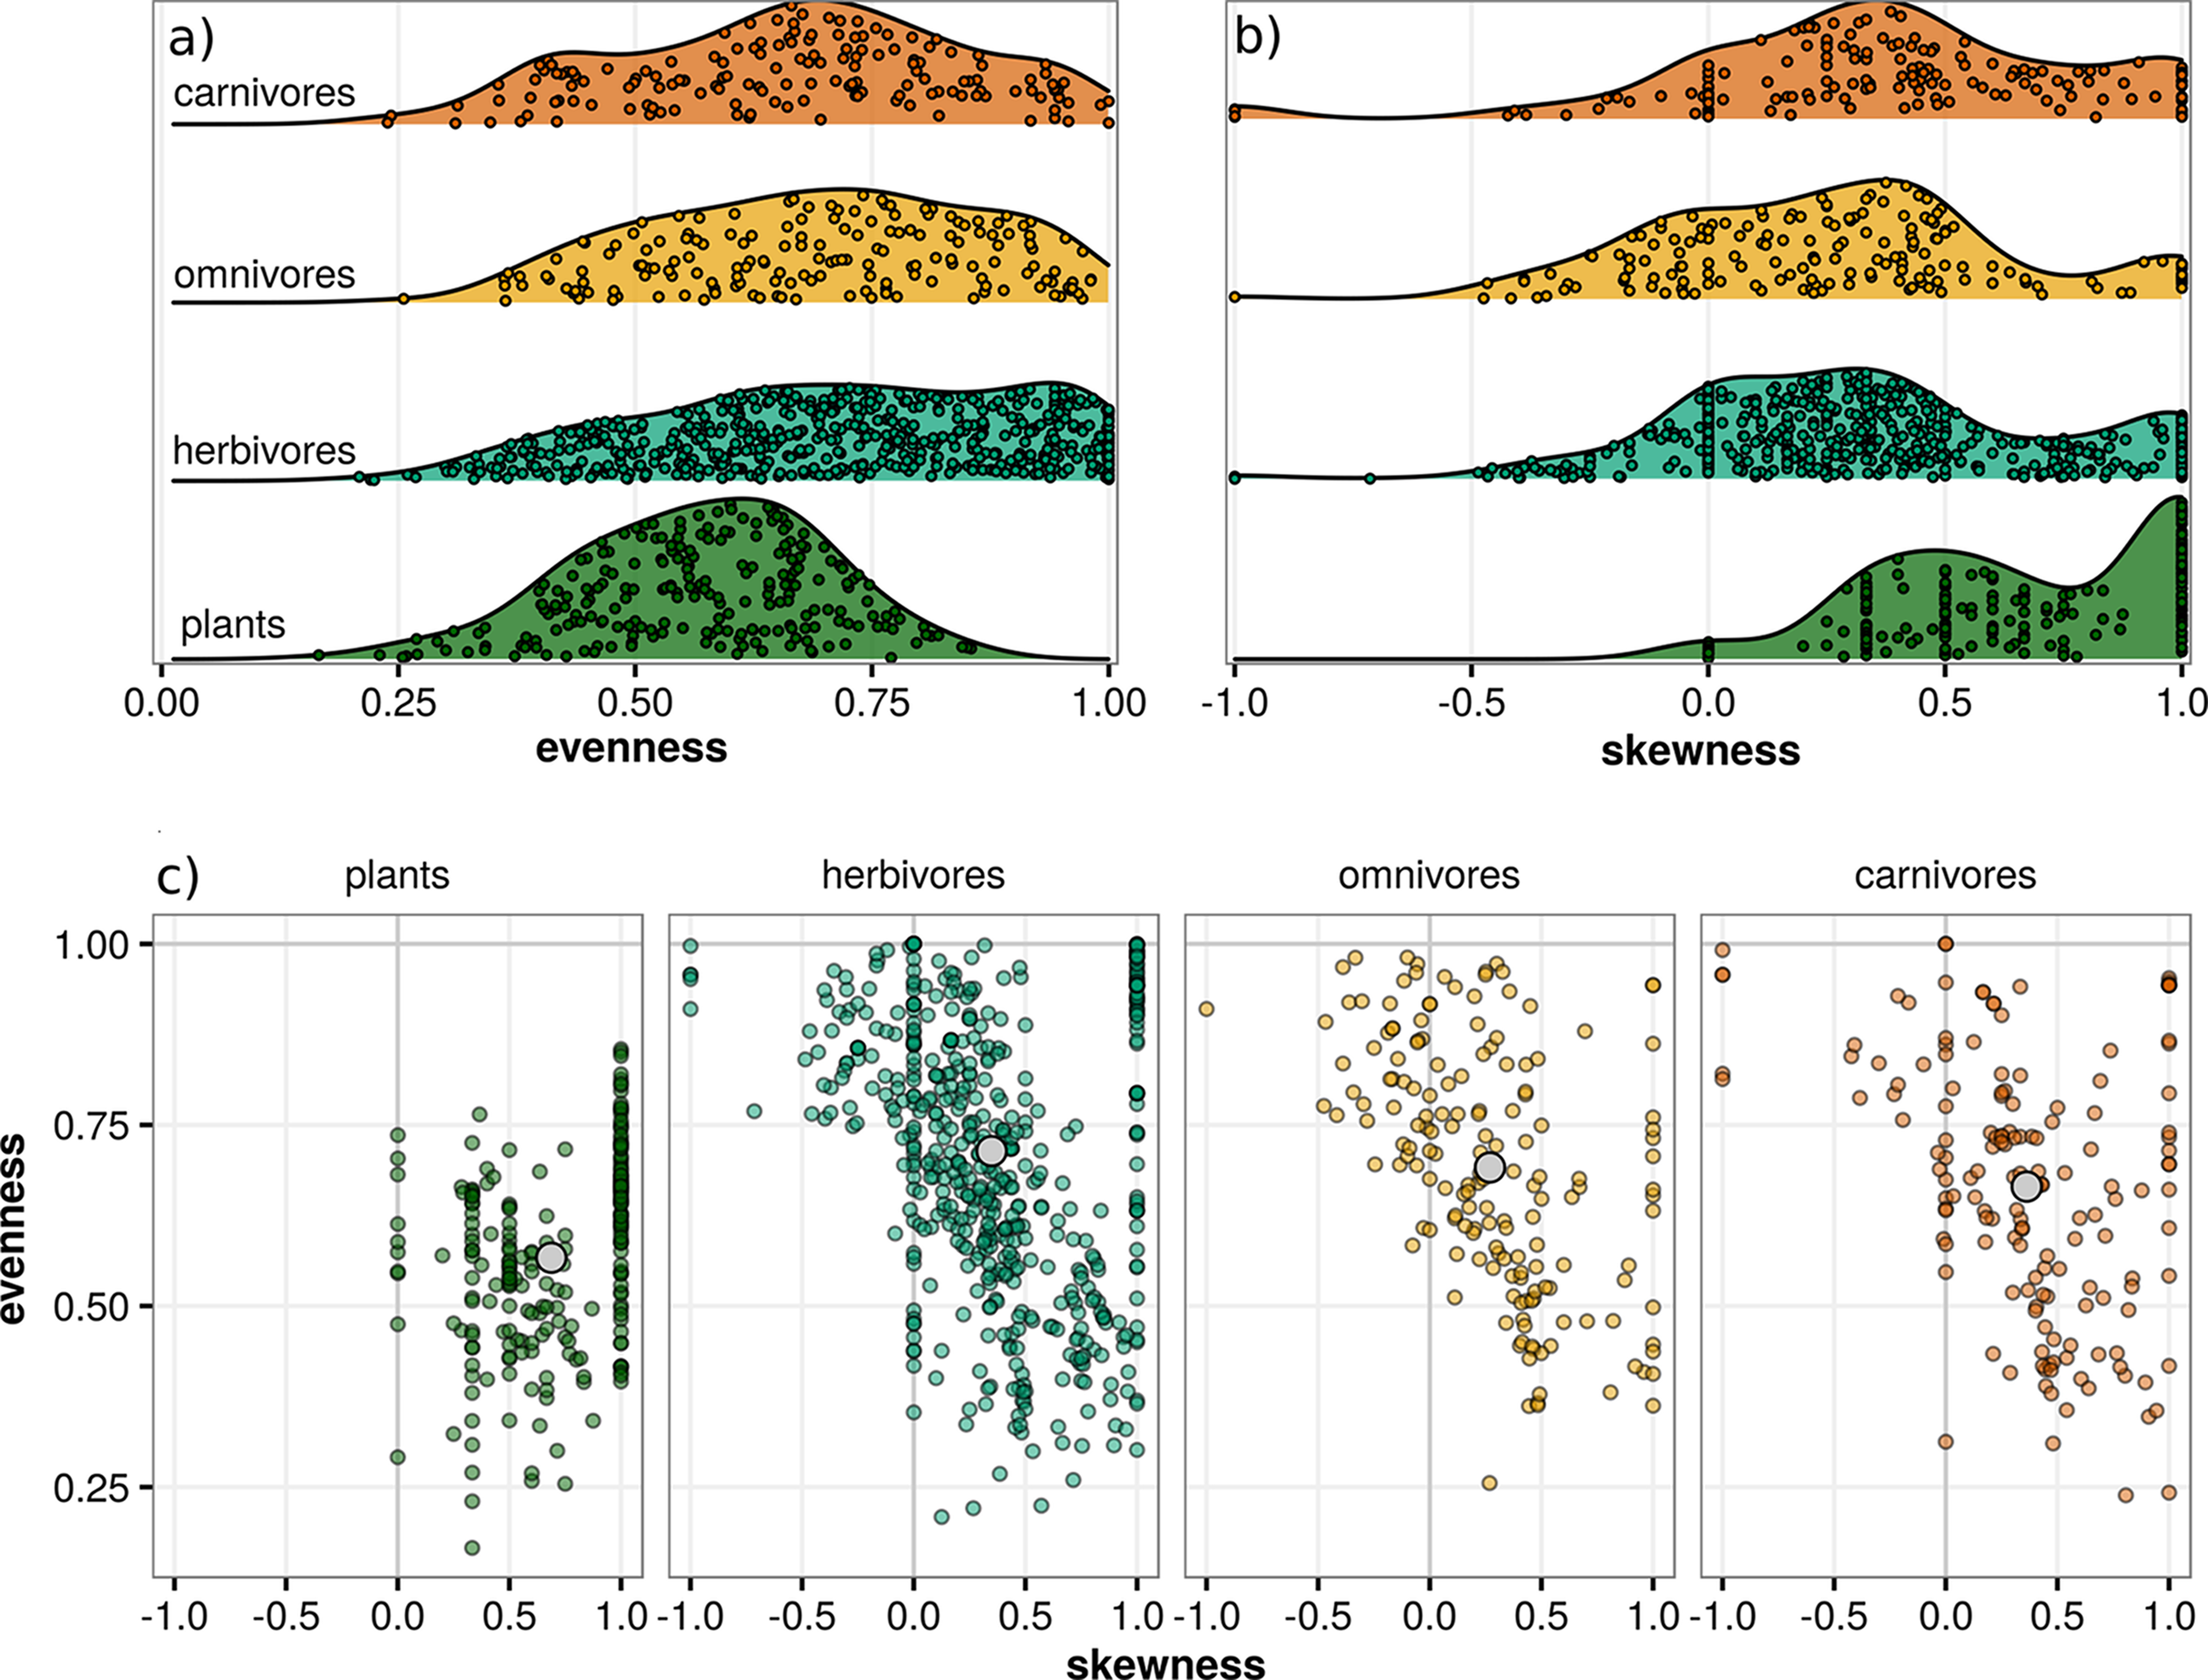
\includegraphics[width=\textwidth]{./Figures/Appendix6_1/Fig_4.png}
\caption[Facilitation impacts]{\color{Gray} Distribution of the net differences between simulations with or without facilitation. Bright colours indicate high values of a metric in the simulations with facilitation relative to the ones without facilitation, and viceversa for darker shades. Note that the colour scales in the three panels are not equivalent; this is due to the different ranges of the differences among metrics.}
\label{fig:figApp6.1.4}
\end{figure}
